% !TeX root = ../main.tex
% Add the above to each chapter to make compiling the PDF easier in some editors.

\chapter{Analysis}

In this chapter, we study functions $f: \sS \to \R$ where $\sS \subseteq \R^n$.

\section{First-order Taylor Approximations}

\begin{defn}[Gradient] The \emph{gradient}\index{gradient} of a function $f: \sS \to \R$ at point $\vx \in \sS$ is, \begin{align}
    \grad f(\vx) \defeq \trans{\begin{bmatrix}
        \pdv{f(\vx)}{\vx(1)} & \cdots & \pdv{f(\vx)}{\vx(n)}
    \end{bmatrix}}.
\end{align}
\end{defn}

For a single-variable function $f: \R \to \R$ that is differentiable, we have for any $x, \delta \in \R$, \begin{align*}
    f(x + \delta) = f(x) + \odv{f(x)}{x} + o(|\delta|), \quad \text{where } \lim_{\delta \to 0} \frac{o(|\delta|)}{|\delta|} = 0,
\end{align*} using a first-order Taylor approximation around $x$. We can use a similar approximation when $f$ is a multi-variable function.

\begin{defn}[Fréchet differentiability] A function $f: \sS \to \R$ is \emph{(Fréchet) differentiable}\index{Fréchet differentiability} at $\vx \in \sS$ if there exists $\vg \in \R^n$ such that, \begin{align}
    \lim_{\substack{\vdelta \in \R^n \\ \vdelta \to \vZero}} \frac{|f(\vx + \vdelta) - (f(\vx) + \trans{\vg}\vdelta)|}{\norm{\vdelta}_2} = 0.
\end{align}
\end{defn}\noindent Here, $\vg$ can be understood as a candidate for $\grad f(\vx)$ and $f(\vx) + \trans{\vg}\vdelta$ is a linear approximation of $f$ around $\vx$.

This notion of differentiability is equivalent to, \begin{align}
    f(\vx + \vdelta) = f(\vx) + \trans{\grad f(\vx)}\vdelta + o(\norm{\vdelta}_2),
\end{align} for any $\vx, \vdelta \in \R^n$. This is also called a \emph{first-order expansion}\index{first-order expansion} of $f$.

\begin{defn}[Continuous differentiability] We say that $f : \sS \to \R$ is \emph{continuously differentiable}\index{continuously differentiability} on $\sS$ if it is differentiable and its gradient is continuous on $\sS$.
\end{defn}
\begin{lem} A differentiable and convex function $f$, whose domain $\sS \subseteq \R^n$ is open and convex, is always continuously differentiable.
\end{lem}

\begin{thm}[Taylor's theorem]\index{Taylor's theorem} If $f: \sS \to \R$ is continuously differentiable, then for all $\vx, \vy \in \R^n$, \begin{align}
    f(\vy) = f(\vx) + \trans{\grad f(\vz)}(\vy - \vx),
\end{align} for some $\vz \in [\vx, \vy] \defeq \{\theta\vx + (1-\theta)\vy \mid \theta \in [0,1]\}$.
\end{thm}\begin{marginfigure}
\centering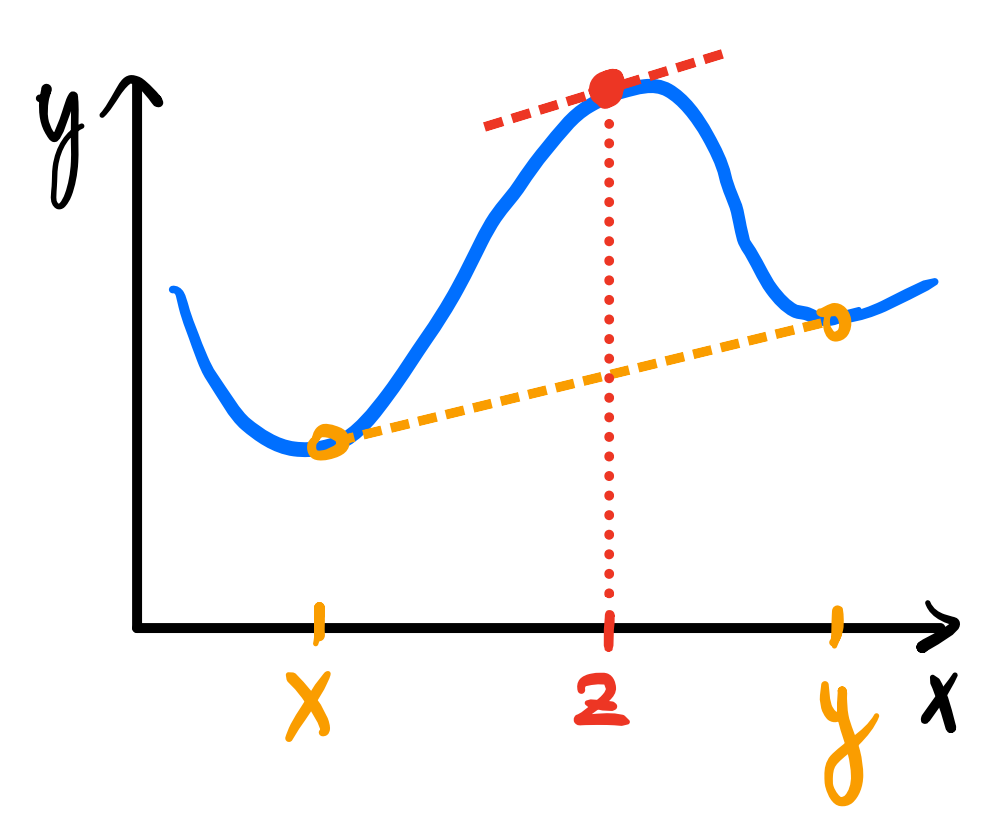
\includegraphics[width=3cm]{notes/figures/taylors_theorem.png}
\caption{Illustration of Taylor's theorem. The affine approximation is shown in orange.}
\end{marginfigure}\noindent Taylor's theorem implies that $f$ can be approximated by the affine function, \begin{align*}
    \vy \to f(\vx) + \trans{\grad f(\vx)}(\vy - \vx),
\end{align*} when $\vy$ is ``close to'' $\vx$.

\section{Directional Derivatives}

\begin{defn}[Directional derivative] Let $f: \sS \to \R$ be differentiable at $\vx \in \R^n$. Given $\vd \in \R^n$, the \emph{directional derivative}\index{directional derivative} of $f$ at $\vx$ in the direction $\vd$ is, \begin{align}
    D f(\vx)[\vd] \defeq \lim_{\lambda \to 0} \frac{f(\vx + \lambda\vd) - f(\vx)}{\lambda}.
\end{align}
\end{defn}

\begin{lem} $D f(\vx)[\vd] = \trans{\grad f(\vx)}\vd$.
\end{lem}
\begin{proof} Using a first-order expansion, we have, \begin{align*}
    f(\vx + \lambda\vd) = f(\vx) + \lambda \trans{\grad f(\vx)}\vd + o(\lambda \norm{\vd}_2).
\end{align*} Dividing by $\lambda$ yields, \begin{align*}
    \frac{f(\vx + \lambda\vd) - f(\vx)}{\lambda} = \trans{\grad f(\vx)}\vd + \underbrace{\frac{o(\lambda\norm{\vd}_2)}{\lambda}}_{\to 0}.
\end{align*} Taking the limit $\lambda \to 0$ gives the desired result.
\end{proof}

\section{Conditions for Optimality}

\begin{defn}[Stationary point] Given a function $f: \sS \to \R$, a point $\vx \in \sS$ where $\grad f(\vx) = 0$ is called a \emph{stationary point}\index{stationary point} of $f$.\footnote{Being a stationary point is not sufficient for optimality. Take for example the point $x \defeq 0$ of $f(x) \defeq x^3$.}
\end{defn}

\begin{lem}
If $\vx \in \sS$ is a local extremum of a differentiable function $f: \sS \to \R$, then $\grad f(\vx) = 0$.\footnote{Here it is important that we have chosen $\sS \subseteq \R^n$ to be open. When $\sS$ is not open, an extremum could be on the boundary of the domain, where the gradient is non-zero.}
\end{lem}
\begin{proof}
    Assume $\vx$ is a local minimum of $f$. Then, for all $\vd \in \R^n$ and for all small enough $\lambda \in R$, we have $f(\vx) \leq f(\vx + \lambda\vd)$, so, \begin{align*}
        0 &\leq f(\vx + \lambda\vd) - f(\vx) \\
        &= \lambda \trans{\grad f(\vx)}\vd + o(\lambda\norm{\vd}_2). \margintag{using a first-order expansion of $f$ around $x$}
    \end{align*} Dividing by $\lambda$ and taking the limit $\lambda \to 0$, we obtain, \begin{align*}
        0 \leq \trans{\grad f(\vx)}\vd + \underbrace{\frac{o(\lambda\norm{\vd}_2)}{\lambda}}_{\to 0} \to \trans{\grad f(\vx)}\vd.
    \end{align*} Take $\vd \defeq - \grad f(\vx)$.\footnote{We can only take this step because we assumed that $\sS$ is open.} Then, \begin{align*}
        0 \leq - \norm{\grad f(\vx)}_2^2,
    \end{align*} so $\grad f(\vx) = 0$.
\end{proof}

\section{Second-order Taylor Approximations}